\documentclass[../mathNotesPreamble]{subfiles}
\begin{document}
%\relscale{1.4}
  \section{12.1: Parametric Equations}

  \noindent We've already seen a parametric equation represented by the unit circle. Here, we have
    \[x(\theta)=\cos(\theta) \textnormal{ and } y(\theta)=\sin(\theta), \textnormal{ where } 0\leq\theta\leq 2\pi\]
  \vspace*{\stretch{1}}
  \begin{center}
    \newcommand{\lCol}{gray!90}
    \normalsize
    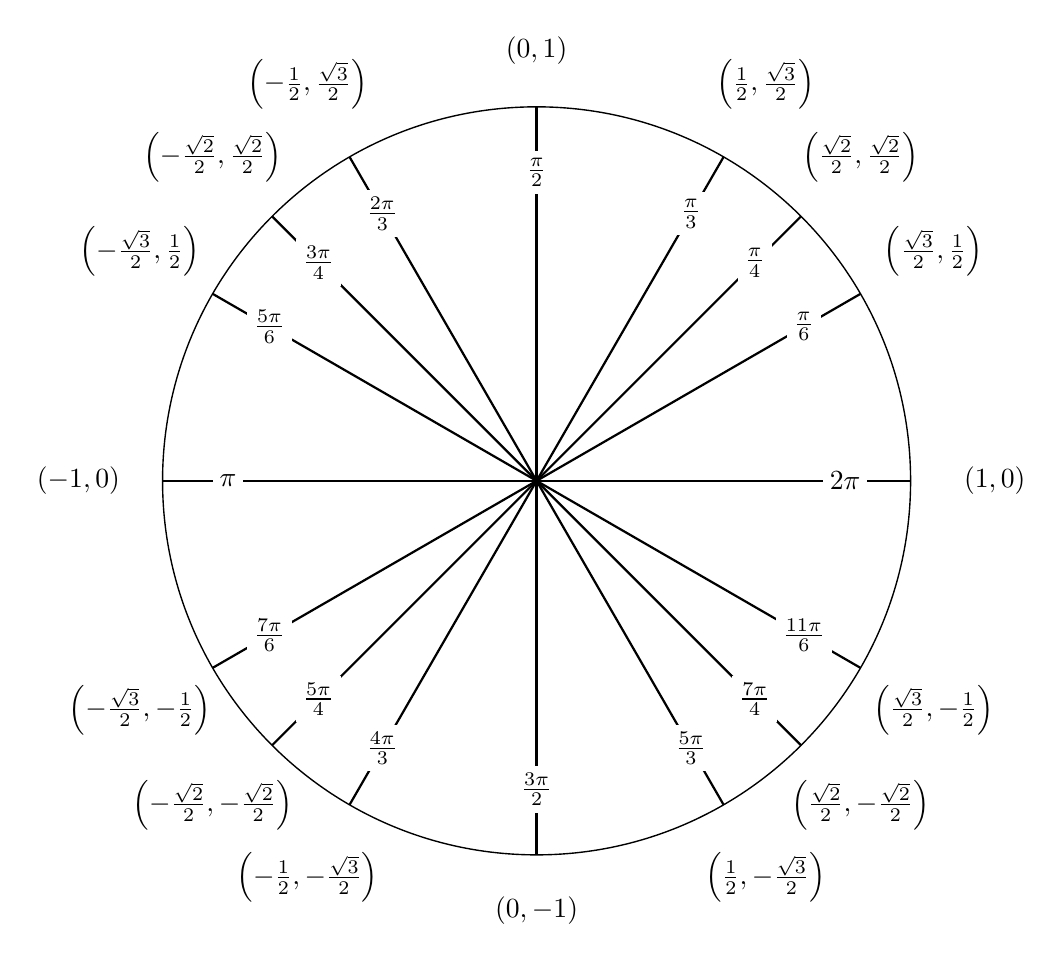
\begin{tikzpicture}[scale=1.0, line width=0.8pt, declare function={
      cRad=4.75; rRad=0.825*cRad; tRad=1.225*cRad;}]
      \draw[line width=0.5pt] (0,0) circle(cRad);
      \foreach \x/\xtext in {
        30/\frac{\pi}{6},    45/\frac{\pi}{4},   60/\frac{\pi}{3},    90/\frac{\pi}{2},
        120/\frac{2\pi}{3}, 135/\frac{3\pi}{4}, 150/\frac{5\pi}{6},  180/\pi,
        210/\frac{7\pi}{6}, 225/\frac{5\pi}{4}, 240/\frac{4\pi}{3},  270/\frac{3\pi}{2},
        300/\frac{5\pi}{3}, 315/\frac{7\pi}{4}, 330/\frac{11\pi}{6}, 360/2\pi}{
          \draw[\lCol] (0cm,0cm) -- (\x:cRad);
          \draw (\x:rRad) node[fill=white, inner sep=2.5pt] {$\xtext$};
        }
    \foreach \x/\xtext/\y in {
      % the coordinates for the first quadrant
      30/\frac{\sqrt{3}}{2}/\frac{1}{2},
      45/\frac{\sqrt{2}}{2}/\frac{\sqrt{2}}{2},
      60/\frac{1}{2}/\frac{\sqrt{3}}{2},
      % the coordinates for the second quadrant
      150/-\frac{\sqrt{3}}{2}/\frac{1}{2},
      135/-\frac{\sqrt{2}}{2}/\frac{\sqrt{2}}{2},
      120/-\frac{1}{2}/\frac{\sqrt{3}}{2},
      % the coordinates for the third quadrant
      210/-\frac{\sqrt{3}}{2}/-\frac{1}{2},
      225/-\frac{\sqrt{2}}{2}/-\frac{\sqrt{2}}{2},
      240/-\frac{1}{2}/-\frac{\sqrt{3}}{2},
      % the coordinates for the fourth quadrant
      330/\frac{\sqrt{3}}{2}/-\frac{1}{2},
      315/\frac{\sqrt{2}}{2}/-\frac{\sqrt{2}}{2},
      300/\frac{1}{2}/-\frac{\sqrt{3}}{2}}
        \draw (\x:tRad) node {$\left(\xtext,\y\right)$};
        \draw (-tRad,0cm) node{$(-1,0)$}
              (tRad,0cm)  node{$(1,0)$}
              (0cm,-cRad*1.15) node{$(0,-1)$}
              (0cm,cRad*1.15)  node{$(0,1)$};
    \end{tikzpicture}
  \end{center}
  \vspace*{\stretch{1}}

  \begin{defn*}[Positive Orientation]
    The direction in which a parametric curve is generated as the parameter increases is called the \textbf{positive orientation} of the curve (and is indicated by arrows on the curve).
  \end{defn*}
  \pagebreak

  \begin{ex*}[\textcolor{blue}{LC 32.1-32.2}]
    Consider the parametric equations
      \[x=3\cos(t),\ y=3\sin(t); \pi\leq t\leq 2\pi\]
  \end{ex*}
  \begin{tasks}[after-item-skip=\stretch{1}, label=,item-indent=0pt](1)
    \task Eliminate the parameter $t$ and rewrite as a function of $x$ and $y$.
    \task Graph the equation found above indicating the positive orientation.
  \end{tasks}
  \begin{center}
    \begin{tikzpicture}[scale=1.1]
      \begin{axis}[
        axis lines=center,
        axis line style={black,->},
        xmin=-4.5, xmax=4.5,
        ymin=-4.5, ymax=4.5,
        xtick={-6,-5,...,6},
        xticklabels={},
        ytick={-6,-5,...,6},
        yticklabels={},
        ticklabel style={font=\footnotesize,inner sep=0.5pt,fill=white,opacity=1.0, text opacity=1},
        xlabel=$x(t)$, xlabel style={at={(ticklabel* cs:1)},anchor=north west},
        ylabel=$y(t)$, ylabel style={at={(ticklabel* cs:1)},anchor=south west},
        every axis plot/.append style={line width=0.95pt, color=blue, samples=100}
        ]
      \end{axis}
    \end{tikzpicture}
  \end{center}
  \pagebreak

  \begin{ex*}[\textcolor{blue}{LC 32.3-32.4}]
    A Ferris wheel has a radius of $20$ m and completes a revolution in the \textbf{clockwise} direction at constant speed in $3$ minutes.  Assume $x$ and $y$ measure the horizontal and vertical positions of a seat on the Ferris wheel relative to a coordinate system whose origin is at the low point of the wheel.  Assume the seat begins moving at the origin.
  \end{ex*}
  \begin{flushright}
    \smash{\raisebox{-\height+1.5\baselineskip}{
    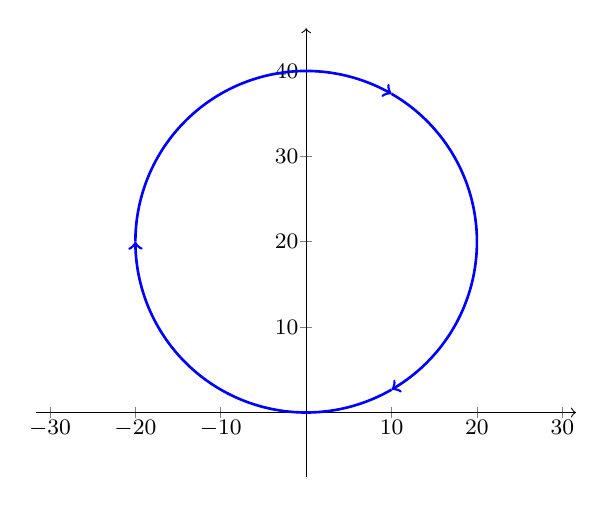
\begin{tikzpicture}[declare function={
      c=0; d=20;}]
      \begin{axis}[
          axis lines=center,
          axis line style={black,->},
          axis equal,
          ymin=-7.5, ymax=45,
          ticklabel style={font=\footnotesize,inner sep=0.5pt,fill=white,opacity=1.0, text opacity=1},
          every axis plot/.append style={line width=0.95pt, color=blue, samples=100}
        ]
        \addplot[<-, data cs=polar, domain=-45:15] (x,{2*c*cos(x)+2*d*sin(x)});
        \addplot[<-, data cs=polar, domain=15:75] (x,{2*c*cos(x)+2*d*sin(x)});
        \addplot[<-, data cs=polar, domain=75:135] (x,{2*c*cos(x)+2*d*sin(x)});
      \end{axis}
    \end{tikzpicture}}}
  \end{flushright}
  \vspace*{-1.5\baselineskip}
  \begin{tasks}[after-item-skip=\stretch{1}, label=,item-indent=0pt](1)
    \task \parbox{0.7\linewidth}{What is the domain of $t$ such that the Ferris wheel completes one revolution?}
    \task $x(t)$ and $y(t)$ will be parameterized using $\sin(bt)$ and $\cos(bt)$. What is $b$?
    \task What parametric equations describe the path of the seat on the Ferris wheel?
  \end{tasks}
  \vspace*{\stretch{1}}
  \pagebreak

  \begin{thmBox*}[Summary: Parametric Equations of a Line]
    The equations
      \[x=x_0+at,\ y=y_0+bt,\ \textnormal{ for } -\infty<t<\infty,\]
    where $x_0$, $y_0$, $a$, and $b$ are constants with $a\neq 0$, describe a line with slope $\frac{b}{a}$ passing through the point $(x_0,y_0)$. If $a=0$ and $b\neq0$, the line is vertical.
  \end{thmBox*}

  \begin{ex*}
    Find 2 parameterized equations of the line that goes through the points $(3,-4)$ and $(-2,3)$.
  \end{ex*}
  \vspace*{\stretch{1}}

  \begin{ex*}
    Find a parameterized equation for the line segment that connects the points $(3,0)$ and $(-1,3)$.
  \end{ex*}
  \vspace*{\stretch{1}}
  \pagebreak

  \begin{ex*}
    Consider the parametric equations 
      \[x(t)=6-2t \textnormal{ and } y(t)=-2+t,\] 
  \end{ex*}
  \begin{tasks}[after-item-skip=\stretch{0}, label=,item-indent=0pt](1)
    \task Graph the curve indicating the positive orientation
      \begin{center}
        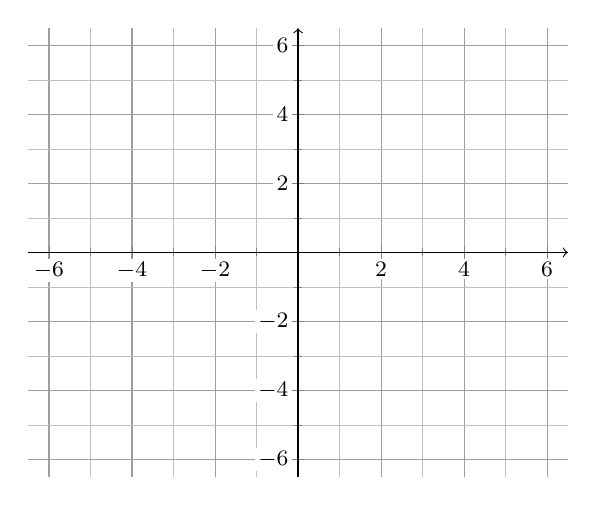
\begin{tikzpicture}[declare function={
          c=0; d=20;}]
          \begin{axis}[
            grid=both, %major,minor
            grid style={line width=0.3pt, draw=gray!60},
            major grid style={line width=0.375pt, draw=gray!75},
            minor grid style={line width=0.15pt, draw=gray!50},
            axis lines=center,
            axis line style={black,->},
            xmin=-6.5, xmax=6.5,
            ymin=-6.5, ymax=6.5,
            minor x tick num=1,
            minor y tick num=1,
            ticklabel style={font=\footnotesize,inner sep=1.15pt,fill=white,opacity=1.0, text opacity=1},
            every axis plot/.append style={line width=0.95pt, color=blue, samples=100}
            ]
          \end{axis}
        \end{tikzpicture}
      \end{center}
    \task Eliminate the parameter to find an equation in $x$ and $y$.
  \end{tasks}
  \vspace*{\stretch{1}}
  \pagebreak

  \begin{ex*}[\textcolor{blue}{LC 32.5-32.7}]
    Consider the parametric equations
      \[x=1+e^{2t}\textnormal{ and } y=e^t,\]
  \end{ex*}
  \begin{tasks}[after-item-skip=\stretch{1}, label=,item-indent=0pt](1)
    \task Eliminate the parameter to find an equation in $x$ and $y$
    \task Graph the curve indicating the positive orientation
      \begin{center}
        \smash{\raisebox{-\height+\baselineskip}{
          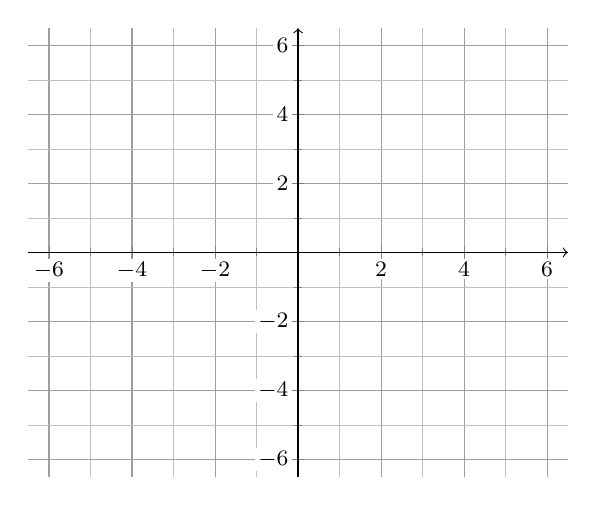
\begin{tikzpicture}[scale=1.0]
            \begin{axis}[
              grid=both, %major,minor
              grid style={line width=0.3pt, draw=gray!60},
              major grid style={line width=0.375pt, draw=gray!75},
              minor grid style={line width=0.15pt, draw=gray!50},
              axis lines=center,
              axis line style={black,->},
              xmin=-6.5, xmax=6.5,
              ymin=-6.5, ymax=6.5,
              minor x tick num=1,
              minor y tick num=1,
              ticklabel style={font=\footnotesize,inner sep=1.15pt,fill=white,opacity=1.0, text opacity=1},
              every axis plot/.append style={line width=0.95pt, color=blue, samples=100}
              ]
            \end{axis}
          \end{tikzpicture}
        }}
      \end{center}
    \task Which of the following parametric equations are equivalent?
    \begingroup
    \addtolength{\jot}{5mm}
    \begin{alignat*}{3}
      x&=2t^2, \hspace*{15mm} &y&=4+t;\hspace*{15mm} &-4\leq{}& t\leq 4\\
      x&=2t^4, &y&=4+t^2; &-2\leq{}& t\leq 2\\
      x&=2t^{2/3}, &y&=4+t^{1/3}; &-64\leq{}& t\leq 64
    \end{alignat*}
    \endgroup
  \end{tasks}
  \pagebreak

  \begin{thmBox*}[Theorem 12.1: Derivative for Parametric Curves]
    Let $x=f(t)$ and $y=g(t)$, where $f$ and $g$ are differentiable on an interval $[a,b]$. Then the slope of the line tangent to the curve at the point corresponding to $t$ is
      \[\frac{dy}{dx}=\frac{dy/dt}{dx/dt}=\frac{g'(t)}{f'(t)},\]
    provided $f'(t)\neq 0$.
  \end{thmBox*}
  \begin{ex*}[\textcolor{blue}{LC 32.8-32.9}]
    Consider the parametric equations
      \[x=\sqrt{t},\qquad y=2t,\]
  \end{ex*}
  \begin{tasks}[after-item-skip=\stretch{1}, label=,item-indent=0pt](1)
    \task Find $\dfrac{dy}{dt}$.
    \task Find the equation of the line tangent to the curve at $t=4$.
  \end{tasks}
  \vspace*{\stretch{1}}
  \pagebreak

  \begin{defn*}[Arc Length for Curves Defined by Parametric Equations]
    Consider the curve described by the parametric equations $x=f(t)$, $y=g(t)$, where $f'$ and $g'$ are continuous, and the curve is traversed once for $a\leq t\leq b$. The \textbf{arc length} of the curve between $\parens{f(a),g(a)}$ and $\parens{f(b),g(b)}$ is
      \[L=\int_a^b \sqrt{f'(t)^2+g'(t)^2}\,dt.\]
  \end{defn*}

  \begin{ex*}[\textcolor{blue}{LC 33.1-33.2}]
    Find the arc length of the curve given by $x=6t^2$, $y=2t^3$, for $0\leq t\leq 4$.
  \end{ex*}
  \vspace*{\stretch{1}}
  \pagebreak

  \begin{ex*}
    Suppose the function $y=h(x)$ is nonnegative and continuous on $[\alpha,\beta]$, which implies that the area bounded by the graph of $h$ and the $x$-axis on $[\alpha,\beta]$ equals $\int_\alpha^\beta h(x)\,dx$ or $\int_\alpha^\beta y\,dx$. If the graph of $y=h(x)$ on $[\alpha,\beta]$ is traced exactly once by the parametric equations $x=f(t)$, $y=g(t)$, for $a\leq t\leq b$, then it follows by substitution that the area bounded by $h$ is
      \[\int_\alpha^\beta h(x)\,dx=\int_a^b g(t)f'(t)\,dt \textnormal{ if }\alpha=f(a) \textnormal{ and } \beta=f(b)\]
    Find the area under one arch of the cycloid $x=3(t-\sin(t))$, $y=3(1-\cos(t))$.
  \end{ex*}
  \begin{center}
    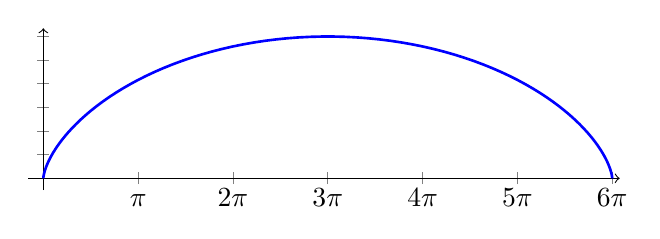
\begin{tikzpicture}
      \begin{axis}[
        axis lines=center,
        axis line style={black,->},
        xmin=-0.5, xmax=6*pi+0.25,
        ymin=-0.5, ymax=6.35,
        xtick={0,pi,2*pi,3*pi,4*pi,5*pi,6*pi},
        xticklabels={$0$,$\vphantom{2}\pi$,$2\pi$,$3\pi$,$4\pi$,$5\pi$,$6\pi$},
        ytick={-6,-5,...,6},
        yticklabels={},
        ticklabel style={font=\normalsize,inner sep=1.5pt,fill=white,opacity=1.0, text opacity=1},
        every axis plot/.append style={line width=0.95pt, color=blue, samples=100},
        width=0.75\linewidth, height=0.3\linewidth
        ]
        \addplot[-, domain=0:2*pi] ({3*(x-sin(deg(x))},{3*(1-cos(deg(x))});
      \end{axis}
    \end{tikzpicture}
  \end{center}
  \vspace*{\stretch{1}}
  \pagebreak
  
  \begin{ex*}[\textcolor{blue}{33.3} Surface area]
    Let $C$ be the curve $x=f(t)$, $y=g(t)$, for $a\leq t\leq b$, where $f'$ and $g'$ are continuous on $[a,b]$ and $C$ does not intersect itself, except possibly at its endpoints. If $g$ is nonnegative on $[a,b]$, then the area of the surface obtained by revolving $C$ about the $x$-axis is
      \[S=\int_a^b 2\pi g(t)\sqrt{f'(t)^2+g'(t)^2}\,dt.\]
    Setup the integral used to find the area of the surface obtained by revolving the curve $x=t\sin(t)$, $y=t\cos(t)$, for $0\leq t\leq \pi/2$, about the $x$-axis.
  \end{ex*}
  \vspace*{\stretch{1}}
  \pagebreak

\end{document}
